\section{Functor $\mathrm{Ext}$ and $\mathrm{Tor}$}
In this section we mention some basic results in Homological Algebra, especially the properties of the functor $\mathrm{Ext}$ and $\mathrm{Tor}$. This section will be used in commutative algebra.\par
Our main reference is Dummit and Foote \textit{Abstract Algebra}.
\begin{definition}
Let $\mathcal{C}$ be a sequence of abelian group homomorphisms: 
$$
0\longrightarrow C^0\overset{d_1}{\longrightarrow}C^1\longrightarrow \cdots \longrightarrow C^{n-1}\overset{d_n}{\longrightarrow}C^n\overset{d_{n+1}}{\longrightarrow}\cdots .
$$
The sequence $\mathcal{C}$ is called a \textbf{cochain complex} if the composition of any two successive maps is zero, i.e. $d_{n+1}\circ d_n=0$ for all $n$. If $\mathcal{C}$ is a cochain complex, its $n$-th \textbf{cohomology group} is the quotient group $\mathrm{Ker}d_{n+1}/\mathrm{Im}d_n$, and is denoted by $H^n(\mathcal{C})$.
\end{definition}
There is completely a dual version of the cochain complex: Let $\mathcal{C}$ be a sequence of abelian group homomorphisms: 
$$
\cdots \overset{d_{n+1}}{\longrightarrow}C^n\overset{d_n}{\longrightarrow}C^{n-1}\longrightarrow \cdots \longrightarrow C^1\overset{d_1}{\longrightarrow}C^0\longrightarrow 0,
$$
then $\mathcal{C}$ is called a \textbf{chain complex} and its \textbf{homology group} is defined to be $H^n(\mathcal{C})=\mathrm{Ker}d_n/\mathrm{Im}d_{n+1}$.  For chain complexes the notation is often chosen so that the indices appear as subscripts and are decreasing, whereas for cochain complexes the indices are superscripts and are increasing. We shall instead use a uniform notation for the maps on both, since it will be clear from the context whether we are dealing with a chain or a cochain complex.\par
In this section we shall focus on cochain complex and cohomology groups, while for chain complex and homology groups we almost always have a similar statement.\par
\begin{definition}
Let $\mathcal{A}=\{A^n\}$ and $\mathcal{B}=\{B^n\}$ be cochain complexes. A \textbf{homomorphism of complexes} $\alpha:\mathcal{A}\to\mathcal{B}$ is a set of homomorphisms $\alpha_n:A^n\to B^n$ such that for every $n$ the diagram commutes: 
\begin{center}


\tikzset{every picture/.style={line width=0.75pt}} %set default line width to 0.75pt        

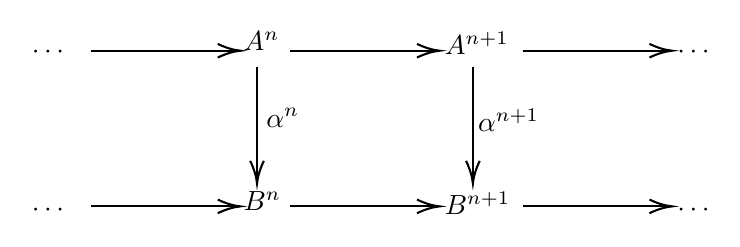
\begin{tikzpicture}[x=0.75pt,y=0.75pt,yscale=-1,xscale=1]
%uncomment if require: \path (0,476); %set diagram left start at 0, and has height of 476

%Straight Lines [id:da7524638160806612] 
\draw    (240,168) -- (310,168) ;
\draw [shift={(312,168)}, rotate = 180] [color={rgb, 255:red, 0; green, 0; blue, 0 }  ][line width=0.75]    (10.93,-3.29) .. controls (6.95,-1.4) and (3.31,-0.3) .. (0,0) .. controls (3.31,0.3) and (6.95,1.4) .. (10.93,3.29)   ;
%Straight Lines [id:da9376306200838702] 
\draw    (224,176) -- (224,230) ;
\draw [shift={(224,232)}, rotate = 270] [color={rgb, 255:red, 0; green, 0; blue, 0 }  ][line width=0.75]    (10.93,-3.29) .. controls (6.95,-1.4) and (3.31,-0.3) .. (0,0) .. controls (3.31,0.3) and (6.95,1.4) .. (10.93,3.29)   ;
%Straight Lines [id:da8096263720008363] 
\draw    (328,176) -- (328,230) ;
\draw [shift={(328,232)}, rotate = 270] [color={rgb, 255:red, 0; green, 0; blue, 0 }  ][line width=0.75]    (10.93,-3.29) .. controls (6.95,-1.4) and (3.31,-0.3) .. (0,0) .. controls (3.31,0.3) and (6.95,1.4) .. (10.93,3.29)   ;
%Straight Lines [id:da5328330870122056] 
\draw    (240,243) -- (310,243) ;
\draw [shift={(312,243)}, rotate = 180] [color={rgb, 255:red, 0; green, 0; blue, 0 }  ][line width=0.75]    (10.93,-3.29) .. controls (6.95,-1.4) and (3.31,-0.3) .. (0,0) .. controls (3.31,0.3) and (6.95,1.4) .. (10.93,3.29)   ;
%Straight Lines [id:da5398916676799472] 
\draw    (352,168) -- (422,168) ;
\draw [shift={(424,168)}, rotate = 180] [color={rgb, 255:red, 0; green, 0; blue, 0 }  ][line width=0.75]    (10.93,-3.29) .. controls (6.95,-1.4) and (3.31,-0.3) .. (0,0) .. controls (3.31,0.3) and (6.95,1.4) .. (10.93,3.29)   ;
%Straight Lines [id:da7781687909512891] 
\draw    (352,243) -- (422,243) ;
\draw [shift={(424,243)}, rotate = 180] [color={rgb, 255:red, 0; green, 0; blue, 0 }  ][line width=0.75]    (10.93,-3.29) .. controls (6.95,-1.4) and (3.31,-0.3) .. (0,0) .. controls (3.31,0.3) and (6.95,1.4) .. (10.93,3.29)   ;
%Straight Lines [id:da5151373079469965] 
\draw    (144,243) -- (214,243) ;
\draw [shift={(216,243)}, rotate = 180] [color={rgb, 255:red, 0; green, 0; blue, 0 }  ][line width=0.75]    (10.93,-3.29) .. controls (6.95,-1.4) and (3.31,-0.3) .. (0,0) .. controls (3.31,0.3) and (6.95,1.4) .. (10.93,3.29)   ;
%Straight Lines [id:da03071894686354426] 
\draw    (144,168) -- (214,168) ;
\draw [shift={(216,168)}, rotate = 180] [color={rgb, 255:red, 0; green, 0; blue, 0 }  ][line width=0.75]    (10.93,-3.29) .. controls (6.95,-1.4) and (3.31,-0.3) .. (0,0) .. controls (3.31,0.3) and (6.95,1.4) .. (10.93,3.29)   ;

% Text Node
\draw (216,157.4) node [anchor=north west][inner sep=0.75pt]    {$A^{n}$};
% Text Node
\draw (313,157.4) node [anchor=north west][inner sep=0.75pt]    {$A^{n+1}$};
% Text Node
\draw (216,234.4) node [anchor=north west][inner sep=0.75pt]    {$B^{n}$};
% Text Node
\draw (313,234.4) node [anchor=north west][inner sep=0.75pt]    {$B^{n+1}$};
% Text Node
\draw (227,194.4) node [anchor=north west][inner sep=0.75pt]    {$\alpha ^{n}$};
% Text Node
\draw (329,194.4) node [anchor=north west][inner sep=0.75pt]    {$\alpha ^{n+1}$};
% Text Node
\draw (114,164.4) node [anchor=north west][inner sep=0.75pt]    {$\cdots $};
% Text Node
\draw (425,164.4) node [anchor=north west][inner sep=0.75pt]    {$\cdots $};
% Text Node
\draw (425,240.4) node [anchor=north west][inner sep=0.75pt]    {$\cdots $};
% Text Node
\draw (114,240.4) node [anchor=north west][inner sep=0.75pt]    {$\cdots $};


\end{tikzpicture}
\end{center}
\end{definition}
We may see that a homomorphism $\alpha:\mathcal{A}\to\mathcal{B}$ of cochain complexes induces group homomorphisms $H^n(\mathcal{A})\to H^n(\mathcal{B})$ for $n\ge 0$ on their respective cohomology groups.\par
Similar to modules, we have the concept of short exact sequences for cochain complexes: 
\begin{definition}
Let $\mathcal{A}=\{A^n\}$, $\mathcal{B}=\{B^n\}$ and $\mathcal{C}=\{C^n\}$ be cochain complexes. A \textbf{short exact sequence} of complexes 
$$
0\longrightarrow \mathcal{A} \overset{\alpha}{\longrightarrow}\mathcal{B} \overset{\beta}{\longrightarrow}\mathcal{C} \longrightarrow 0
$$
is a sequence of homomorphisms of complexes such that 
$$
0\longrightarrow A^n\overset{\alpha _n}{\longrightarrow}B^n\overset{\beta _n}{\longrightarrow}C^n\longrightarrow 0
$$
is short exact for every $n$.
\end{definition}
One of our main features of cochain complexes is that they lead to long exact sequences in cohomology, which is our first main result: 
\begin{theorem}
Let 
$$
0\longrightarrow \mathcal{A} \overset{\alpha}{\longrightarrow}\mathcal{B} \overset{\beta}{\longrightarrow}\mathcal{C} \longrightarrow 0
$$
be a short exact sequence of cochain complexes. Then there is a long exact sequence of cohomology groups: 
$$
0\longrightarrow H^0\left( \mathcal{A} \right) \longrightarrow H^0\left( \mathcal{B} \right) \longrightarrow H^0\left( \mathcal{C} \right) \overset{\delta _0}{\longrightarrow}H^1\left( \mathcal{A} \right) \longrightarrow \cdots ,
$$
where the maps between cohomology groups at each level are naturally defined by Definition A.3 and the maps $\delta_n$ are called the \textbf{connecting homomorphisms}.
\end{theorem}
\begin{proof}
We shall first show that for all $n\in\mathbb{N}$ we have the series 
$$
H^n\left( \mathcal{A} \right) \longrightarrow H^n\left( \mathcal{B} \right) \longrightarrow H^n\left( \mathcal{C} \right) 
$$
is exact. Consider the following commuting diagram: 
\begin{center}


\tikzset{every picture/.style={line width=0.75pt}} %set default line width to 0.75pt        

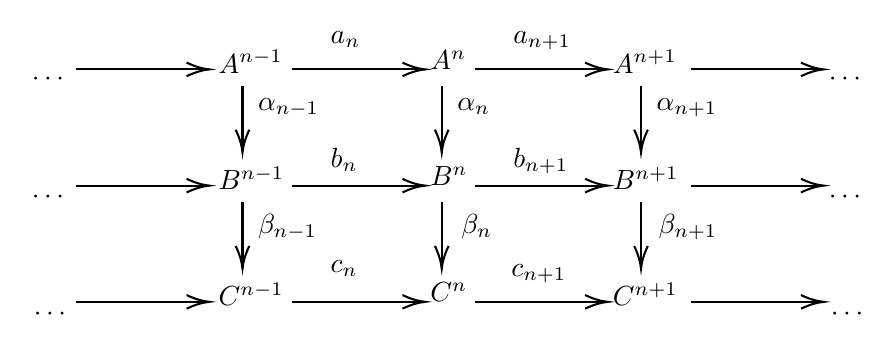
\begin{tikzpicture}[x=0.75pt,y=0.75pt,yscale=-1,xscale=1]
%uncomment if require: \path (0,476); %set diagram left start at 0, and has height of 476

%Straight Lines [id:da2370410467801951] 
\draw    (240,144) -- (302,144) ;
\draw [shift={(304,144)}, rotate = 180] [color={rgb, 255:red, 0; green, 0; blue, 0 }  ][line width=0.75]    (10.93,-3.29) .. controls (6.95,-1.4) and (3.31,-0.3) .. (0,0) .. controls (3.31,0.3) and (6.95,1.4) .. (10.93,3.29)   ;
%Straight Lines [id:da6748831609409329] 
\draw    (328,144) -- (390,144) ;
\draw [shift={(392,144)}, rotate = 180] [color={rgb, 255:red, 0; green, 0; blue, 0 }  ][line width=0.75]    (10.93,-3.29) .. controls (6.95,-1.4) and (3.31,-0.3) .. (0,0) .. controls (3.31,0.3) and (6.95,1.4) .. (10.93,3.29)   ;
%Straight Lines [id:da21398083002271662] 
\draw    (136,144) -- (198,144) ;
\draw [shift={(200,144)}, rotate = 180] [color={rgb, 255:red, 0; green, 0; blue, 0 }  ][line width=0.75]    (10.93,-3.29) .. controls (6.95,-1.4) and (3.31,-0.3) .. (0,0) .. controls (3.31,0.3) and (6.95,1.4) .. (10.93,3.29)   ;
%Straight Lines [id:da6496225329625129] 
\draw    (432,144) -- (494,144) ;
\draw [shift={(496,144)}, rotate = 180] [color={rgb, 255:red, 0; green, 0; blue, 0 }  ][line width=0.75]    (10.93,-3.29) .. controls (6.95,-1.4) and (3.31,-0.3) .. (0,0) .. controls (3.31,0.3) and (6.95,1.4) .. (10.93,3.29)   ;
%Straight Lines [id:da3663728112398783] 
\draw    (240,200) -- (302,200) ;
\draw [shift={(304,200)}, rotate = 180] [color={rgb, 255:red, 0; green, 0; blue, 0 }  ][line width=0.75]    (10.93,-3.29) .. controls (6.95,-1.4) and (3.31,-0.3) .. (0,0) .. controls (3.31,0.3) and (6.95,1.4) .. (10.93,3.29)   ;
%Straight Lines [id:da22592043326464695] 
\draw    (328,200) -- (390,200) ;
\draw [shift={(392,200)}, rotate = 180] [color={rgb, 255:red, 0; green, 0; blue, 0 }  ][line width=0.75]    (10.93,-3.29) .. controls (6.95,-1.4) and (3.31,-0.3) .. (0,0) .. controls (3.31,0.3) and (6.95,1.4) .. (10.93,3.29)   ;
%Straight Lines [id:da832176171749305] 
\draw    (136,200) -- (198,200) ;
\draw [shift={(200,200)}, rotate = 180] [color={rgb, 255:red, 0; green, 0; blue, 0 }  ][line width=0.75]    (10.93,-3.29) .. controls (6.95,-1.4) and (3.31,-0.3) .. (0,0) .. controls (3.31,0.3) and (6.95,1.4) .. (10.93,3.29)   ;
%Straight Lines [id:da05803023373291483] 
\draw    (432,200) -- (494,200) ;
\draw [shift={(496,200)}, rotate = 180] [color={rgb, 255:red, 0; green, 0; blue, 0 }  ][line width=0.75]    (10.93,-3.29) .. controls (6.95,-1.4) and (3.31,-0.3) .. (0,0) .. controls (3.31,0.3) and (6.95,1.4) .. (10.93,3.29)   ;
%Straight Lines [id:da5152767034550616] 
\draw    (240,256) -- (302,256) ;
\draw [shift={(304,256)}, rotate = 180] [color={rgb, 255:red, 0; green, 0; blue, 0 }  ][line width=0.75]    (10.93,-3.29) .. controls (6.95,-1.4) and (3.31,-0.3) .. (0,0) .. controls (3.31,0.3) and (6.95,1.4) .. (10.93,3.29)   ;
%Straight Lines [id:da6061187360861355] 
\draw    (328,256) -- (390,256) ;
\draw [shift={(392,256)}, rotate = 180] [color={rgb, 255:red, 0; green, 0; blue, 0 }  ][line width=0.75]    (10.93,-3.29) .. controls (6.95,-1.4) and (3.31,-0.3) .. (0,0) .. controls (3.31,0.3) and (6.95,1.4) .. (10.93,3.29)   ;
%Straight Lines [id:da32857695821103494] 
\draw    (136,256) -- (198,256) ;
\draw [shift={(200,256)}, rotate = 180] [color={rgb, 255:red, 0; green, 0; blue, 0 }  ][line width=0.75]    (10.93,-3.29) .. controls (6.95,-1.4) and (3.31,-0.3) .. (0,0) .. controls (3.31,0.3) and (6.95,1.4) .. (10.93,3.29)   ;
%Straight Lines [id:da6649666303058066] 
\draw    (432,256) -- (494,256) ;
\draw [shift={(496,256)}, rotate = 180] [color={rgb, 255:red, 0; green, 0; blue, 0 }  ][line width=0.75]    (10.93,-3.29) .. controls (6.95,-1.4) and (3.31,-0.3) .. (0,0) .. controls (3.31,0.3) and (6.95,1.4) .. (10.93,3.29)   ;
%Straight Lines [id:da7321611721199146] 
\draw    (216,152) -- (216,182) ;
\draw [shift={(216,184)}, rotate = 270] [color={rgb, 255:red, 0; green, 0; blue, 0 }  ][line width=0.75]    (10.93,-3.29) .. controls (6.95,-1.4) and (3.31,-0.3) .. (0,0) .. controls (3.31,0.3) and (6.95,1.4) .. (10.93,3.29)   ;
%Straight Lines [id:da04551417993910922] 
\draw    (216,208) -- (216,238) ;
\draw [shift={(216,240)}, rotate = 270] [color={rgb, 255:red, 0; green, 0; blue, 0 }  ][line width=0.75]    (10.93,-3.29) .. controls (6.95,-1.4) and (3.31,-0.3) .. (0,0) .. controls (3.31,0.3) and (6.95,1.4) .. (10.93,3.29)   ;
%Straight Lines [id:da93401112810934] 
\draw    (312,152) -- (312,182) ;
\draw [shift={(312,184)}, rotate = 270] [color={rgb, 255:red, 0; green, 0; blue, 0 }  ][line width=0.75]    (10.93,-3.29) .. controls (6.95,-1.4) and (3.31,-0.3) .. (0,0) .. controls (3.31,0.3) and (6.95,1.4) .. (10.93,3.29)   ;
%Straight Lines [id:da4439225324356606] 
\draw    (312,208) -- (312,238) ;
\draw [shift={(312,240)}, rotate = 270] [color={rgb, 255:red, 0; green, 0; blue, 0 }  ][line width=0.75]    (10.93,-3.29) .. controls (6.95,-1.4) and (3.31,-0.3) .. (0,0) .. controls (3.31,0.3) and (6.95,1.4) .. (10.93,3.29)   ;
%Straight Lines [id:da054029144355214775] 
\draw    (408,152) -- (408,182) ;
\draw [shift={(408,184)}, rotate = 270] [color={rgb, 255:red, 0; green, 0; blue, 0 }  ][line width=0.75]    (10.93,-3.29) .. controls (6.95,-1.4) and (3.31,-0.3) .. (0,0) .. controls (3.31,0.3) and (6.95,1.4) .. (10.93,3.29)   ;
%Straight Lines [id:da011986524379112184] 
\draw    (408,208) -- (408,238) ;
\draw [shift={(408,240)}, rotate = 270] [color={rgb, 255:red, 0; green, 0; blue, 0 }  ][line width=0.75]    (10.93,-3.29) .. controls (6.95,-1.4) and (3.31,-0.3) .. (0,0) .. controls (3.31,0.3) and (6.95,1.4) .. (10.93,3.29)   ;

% Text Node
\draw (203,133.4) node [anchor=north west][inner sep=0.75pt]    {$A^{n-1}$};
% Text Node
\draw (305,133.4) node [anchor=north west][inner sep=0.75pt]    {$A^{n}$};
% Text Node
\draw (393,133.4) node [anchor=north west][inner sep=0.75pt]    {$A^{n+1}$};
% Text Node
\draw (203,189.4) node [anchor=north west][inner sep=0.75pt]    {$B^{n-1}$};
% Text Node
\draw (305,189.4) node [anchor=north west][inner sep=0.75pt]    {$B^{n}$};
% Text Node
\draw (393,189.4) node [anchor=north west][inner sep=0.75pt]    {$B^{n+1}$};
% Text Node
\draw (203,245.4) node [anchor=north west][inner sep=0.75pt]    {$C^{n-1}$};
% Text Node
\draw (305,245.4) node [anchor=north west][inner sep=0.75pt]    {$C^{n}$};
% Text Node
\draw (393,245.4) node [anchor=north west][inner sep=0.75pt]    {$C^{n+1}$};
% Text Node
\draw (257,124.4) node [anchor=north west][inner sep=0.75pt]    {$a_{n}$};
% Text Node
\draw (345,124.4) node [anchor=north west][inner sep=0.75pt]    {$a_{n+1}$};
% Text Node
\draw (257,180.4) node [anchor=north west][inner sep=0.75pt]    {$b_{n}$};
% Text Node
\draw (257,234.4) node [anchor=north west][inner sep=0.75pt]    {$c_{n}$};
% Text Node
\draw (345,180.4) node [anchor=north west][inner sep=0.75pt]    {$b_{n+1}$};
% Text Node
\draw (344,236.4) node [anchor=north west][inner sep=0.75pt]    {$c_{n+1}$};
% Text Node
\draw (222,156.4) node [anchor=north west][inner sep=0.75pt]    {$\alpha _{n-1}$};
% Text Node
\draw (222,212.4) node [anchor=north west][inner sep=0.75pt]    {$\beta _{n-1}$};
% Text Node
\draw (318,156.4) node [anchor=north west][inner sep=0.75pt]    {$\alpha _{n}$};
% Text Node
\draw (414,156.4) node [anchor=north west][inner sep=0.75pt]    {$\alpha _{n+1}$};
% Text Node
\draw (320,212.4) node [anchor=north west][inner sep=0.75pt]    {$\beta _{n}$};
% Text Node
\draw (415,212.4) node [anchor=north west][inner sep=0.75pt]    {$\beta _{n+1}$};
% Text Node
\draw (113,144.4) node [anchor=north west][inner sep=0.75pt]    {$\cdots $};
% Text Node
\draw (113,201.4) node [anchor=north west][inner sep=0.75pt]    {$\cdots $};
% Text Node
\draw (114,257.4) node [anchor=north west][inner sep=0.75pt]    {$\cdots $};
% Text Node
\draw (497,144.4) node [anchor=north west][inner sep=0.75pt]    {$\cdots $};
% Text Node
\draw (497,201.4) node [anchor=north west][inner sep=0.75pt]    {$\cdots $};
% Text Node
\draw (498,257.4) node [anchor=north west][inner sep=0.75pt]    {$\cdots $};


\end{tikzpicture}
\end{center}
We first show that $\beta\circ\alpha=0$. Suppose $a+\mathrm{Im}a_n\in\mathrm{Ker}a_{n+1}/\mathrm{Im}a_n=H^n(\mathcal{A})$, then 
$$
\beta \circ \alpha \left( a+\mathrm{Im}a_n \right) =\beta \left( \alpha \left( a \right) +\mathrm{Im}b_n \right) =\beta \circ \alpha \left( n \right) +\mathrm{Im}c_n=0\in H^n\left( \mathcal{C} \right) ,
$$
hence we have $\beta\circ\alpha=0$. Now we show that $\mathrm{Im}\alpha=\mathrm{Ker}\beta$. Suppose $b+\mathrm{Im}b_n\in\mathrm{Im}\alpha$, then there exists some $a+\mathrm{Im}a_n\in H^n(\mathcal{A})$ such that $\alpha(a+\mathrm{Im}a_n)=b+\mathrm{Im}b_n$. Hence $\beta\circ\alpha(a+\mathrm{Im}a_n)=\beta(b+\mathrm{Im}b_n)=0$, whence $b+\mathrm{Im}b_n\in\mathrm{Ker}\beta$ and hence $\mathrm{Im}\alpha\subset\mathrm{Ker}\beta$. Conversely, suppose $b=\mathrm{Im}b_n\in\mathrm{Ker}\beta$, then $\beta(b+\mathrm{Im}b_n)=\beta(b)+\mathrm{Im}a_n=0$. Hence there exists some $c^\prime\in C_{n-1}$ such that $c_n(c^\prime)=\beta(b)$. Now by diagram chasing we have $\mathrm{Ker}\beta\subset\mathrm{Im}\alpha$, which finished the proof.\par
We now give the definition of the connecting homomorphism without showing exactness. Suppose $c\in C^n$ is a representation element of $x\in H^n(\mathcal{C})$. Then there is some $b\in B^n$ such that $\beta_n(b)=c$. We may show that there is a unique $a\in A^{n+1}$ such that $\alpha_{n+1}(a)=b_{n+1}(b)$. Define $\delta_n(x)=\overline{a}$, where $\overline{a}$ is the equivalent class of the representation element $a$ in $H^{n+1}(\mathcal{A})$. We omit the details of showing $\delta_n$ is well-defined and a homomorphism.
\end{proof}
\begin{corollary}
Let 
$$
0\longrightarrow \mathcal{A} \overset{\alpha}{\longrightarrow}\mathcal{B} \overset{\beta}{\longrightarrow}\mathcal{C} \longrightarrow 0
$$
be a short exact sequence of cochain complexes. Then if any two of $\mathcal{A}$, $\mathcal{B}$, $\mathcal{C}$ are exact, then so is the third.
\end{corollary}
\begin{proof}
We know that $\mathcal{A}$ is exact if and only if its cohomology group $H^n(\mathcal{A})=0$. Then suppose there are two cochains that are exact, then the third cochain has its cohomology group in an exact sequence with the left and right side both $0$. Therefore the third cohomology group is also zero, which finished the proof.
\end{proof}
We now turn to the introduction on the functor $\mathrm{Ext}$. Suppose $A$ is any $R$-module, a \textbf{projective resolution} of $A$ is an exact sequence 
$$
\cdots \longrightarrow P_n\overset{d_n}{\longrightarrow}P_{n-1}\longrightarrow \cdots \longrightarrow P_0\overset{\varepsilon}{\longrightarrow}A\longrightarrow 0
$$
such that each $P_i$ is a projective $R$-module.\par
We first show that for each $R$-module $A$, there always exists one projective resolution. Let $P_0$ be any free module over $A$ and define an $R$-module homomorphism $\varepsilon$ from $P_0$ to $A$. Clearly we may make $\varepsilon$ surjective so that the sequence is exact. Let $K_0=\mathrm{Ker}\varepsilon$, define $P_1$ be a free module mapping onto the submodule $K_0$ of $P_0$; we may continue this process and obtain a projective resolution. Such a projective resolution is indeed a \textbf{free resolution}.\par
Given a projective resolution, we may form a related sequence by taking homomorphisms of each of the terms into $D$, which gives the following sequence: 
$$
0\longrightarrow \mathrm{Hom}_R\left( A,D \right) \overset{\varepsilon}{\longrightarrow}\mathrm{Hom}_R\left( P_0,D \right) \longrightarrow \cdots \longrightarrow \mathrm{Hom}_R\left( P_n,D \right) \overset{d_n}{\longrightarrow}\mathrm{Hom}_R\left( P_n,D \right) \longrightarrow \cdots .
$$
It has been proved that the sequence above is a cochain complex. The corresponding cohomology group have a special name.
\begin{definition}
Let $A$ and $D$ be $R$-modules. For any projective resolution 
$$
\cdots \longrightarrow P_n\overset{d_n}{\longrightarrow}P_{n-1}\longrightarrow \cdots \longrightarrow P_0\overset{\varepsilon}{\longrightarrow}A\longrightarrow 0,
$$
we have the cochain complex 
\begin{small}
$$
0\longrightarrow \mathrm{Hom}_R\left( A,D \right) \overset{\varepsilon}{\longrightarrow}\mathrm{Hom}_R\left( P_0,D \right) \longrightarrow \cdots \longrightarrow \mathrm{Hom}_R\left( P_n,D \right) \overset{d_n}{\longrightarrow}\mathrm{Hom}_R\left( P_n,D \right) \longrightarrow \cdots .
$$
\end{small}
Define 
$$
\mathrm{Ext}_{R}^{n}\left( A,D \right) =\mathrm{Ker}d_{n+1}/\mathrm{Im}d_n,
$$
where $\mathrm{Ext}_R^0=\mathrm{Ker}d_1$. The group $\mathrm{Ext}_R^n(A,D)$ is called the \textbf{$n$-th cohomology group derived from the functor $\mathrm{Hom}_R(\cdot,D)$}.
\end{definition}
When $R=\mathbb{Z}$, we shall write $\mathrm{Ext}_\mathbb{Z}^n(A,D)$ in short of $\mathrm{Ext}^n(A,D)$.
We shall now show that $\mathrm{Ext}_R^n(A,D)$ is independent of the choice of the projective resolution. We shall prove this with several propositions.
\begin{proposition}
For any $R$-module $A$ we have $\mathrm{Ext}_R^0(A,D)\cong\mathrm{Hom}_R(A,D)$.
\end{proposition}
\begin{proof}
Since the sequence 
$$
\cdots \longrightarrow P_1\overset{d_1}{\longrightarrow}P_0\overset{\varepsilon}{\longrightarrow}A\longrightarrow 0
$$
is exact, it follows that we have the corresponding sequence 
$$
0\longrightarrow \mathrm{Hom}_R\left( A,D \right) \overset{\varepsilon}{\longrightarrow}\mathrm{Hom}_R\left( P_0,D \right) \overset{d_1}{\longrightarrow}\mathrm{Hom}_R\left( P_1,D \right) \longrightarrow \cdots 
$$
is also exact. Therefore 
$$
\mathrm{Ext}_{R}^{0}\left( A,D \right) \cong \mathrm{Ker}d_1=\mathrm{Im}\varepsilon \cong \mathrm{Hom}_R\left( A,D \right) 
$$
is well-defined.
\end{proof}
In order to show that the cohomology groups $\mathrm{Ext}_R^n(A,D)$ are independent of the choice of projective resolution of $A$ we shall need to be able to "compare" resolutions. The next proposition shows that an $R$-module homomorphism from $A$ to $B$ lifts to a homomorphism from a projective resolution of $A$ to a projective resolution of $B$: where the lifting property is one instance where the projectivity of the modules in the resolution is important.
\begin{proposition}
Let $f:A\to A^\prime$ be any homomorphism of $R$-modules and take projective resolutions of $A$ to $A^\prime$, respectively. Then for each $n\ge 0$ there is a lift $f_n$ of $f$ such that the following diagram commutes: 
\begin{center}


\tikzset{every picture/.style={line width=0.75pt}} %set default line width to 0.75pt        

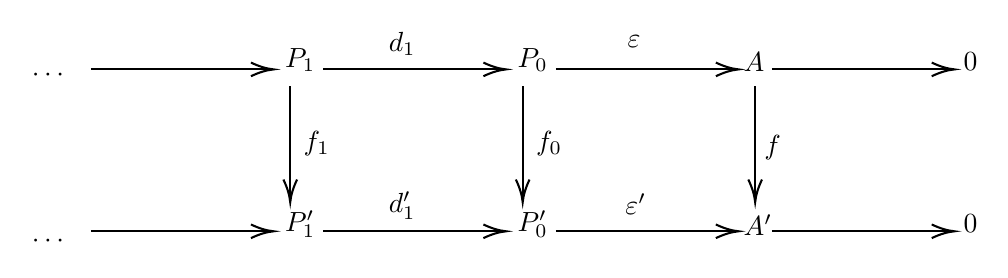
\begin{tikzpicture}[x=0.75pt,y=0.75pt,yscale=-1,xscale=1]
%uncomment if require: \path (0,476); %set diagram left start at 0, and has height of 476

%Straight Lines [id:da8460483192008399] 
\draw    (136,144) -- (222,144) ;
\draw [shift={(224,144)}, rotate = 180] [color={rgb, 255:red, 0; green, 0; blue, 0 }  ][line width=0.75]    (10.93,-3.29) .. controls (6.95,-1.4) and (3.31,-0.3) .. (0,0) .. controls (3.31,0.3) and (6.95,1.4) .. (10.93,3.29)   ;
%Straight Lines [id:da015769832717114296] 
\draw    (248,144) -- (334,144) ;
\draw [shift={(336,144)}, rotate = 180] [color={rgb, 255:red, 0; green, 0; blue, 0 }  ][line width=0.75]    (10.93,-3.29) .. controls (6.95,-1.4) and (3.31,-0.3) .. (0,0) .. controls (3.31,0.3) and (6.95,1.4) .. (10.93,3.29)   ;
%Straight Lines [id:da5890593660239558] 
\draw    (360,144) -- (446,144) ;
\draw [shift={(448,144)}, rotate = 180] [color={rgb, 255:red, 0; green, 0; blue, 0 }  ][line width=0.75]    (10.93,-3.29) .. controls (6.95,-1.4) and (3.31,-0.3) .. (0,0) .. controls (3.31,0.3) and (6.95,1.4) .. (10.93,3.29)   ;
%Straight Lines [id:da4893697163001278] 
\draw    (464,144) -- (550,144) ;
\draw [shift={(552,144)}, rotate = 180] [color={rgb, 255:red, 0; green, 0; blue, 0 }  ][line width=0.75]    (10.93,-3.29) .. controls (6.95,-1.4) and (3.31,-0.3) .. (0,0) .. controls (3.31,0.3) and (6.95,1.4) .. (10.93,3.29)   ;
%Straight Lines [id:da16530627275642962] 
\draw    (136,222) -- (222,222) ;
\draw [shift={(224,222)}, rotate = 180] [color={rgb, 255:red, 0; green, 0; blue, 0 }  ][line width=0.75]    (10.93,-3.29) .. controls (6.95,-1.4) and (3.31,-0.3) .. (0,0) .. controls (3.31,0.3) and (6.95,1.4) .. (10.93,3.29)   ;
%Straight Lines [id:da35122803984286666] 
\draw    (248,222) -- (334,222) ;
\draw [shift={(336,222)}, rotate = 180] [color={rgb, 255:red, 0; green, 0; blue, 0 }  ][line width=0.75]    (10.93,-3.29) .. controls (6.95,-1.4) and (3.31,-0.3) .. (0,0) .. controls (3.31,0.3) and (6.95,1.4) .. (10.93,3.29)   ;
%Straight Lines [id:da27326836730802095] 
\draw    (360,222) -- (446,222) ;
\draw [shift={(448,222)}, rotate = 180] [color={rgb, 255:red, 0; green, 0; blue, 0 }  ][line width=0.75]    (10.93,-3.29) .. controls (6.95,-1.4) and (3.31,-0.3) .. (0,0) .. controls (3.31,0.3) and (6.95,1.4) .. (10.93,3.29)   ;
%Straight Lines [id:da5307504663973357] 
\draw    (464,222) -- (550,222) ;
\draw [shift={(552,222)}, rotate = 180] [color={rgb, 255:red, 0; green, 0; blue, 0 }  ][line width=0.75]    (10.93,-3.29) .. controls (6.95,-1.4) and (3.31,-0.3) .. (0,0) .. controls (3.31,0.3) and (6.95,1.4) .. (10.93,3.29)   ;
%Straight Lines [id:da7525902918596272] 
\draw    (232,152) -- (232,206) ;
\draw [shift={(232,208)}, rotate = 270] [color={rgb, 255:red, 0; green, 0; blue, 0 }  ][line width=0.75]    (10.93,-3.29) .. controls (6.95,-1.4) and (3.31,-0.3) .. (0,0) .. controls (3.31,0.3) and (6.95,1.4) .. (10.93,3.29)   ;
%Straight Lines [id:da9644455390597471] 
\draw    (344,152) -- (344,206) ;
\draw [shift={(344,208)}, rotate = 270] [color={rgb, 255:red, 0; green, 0; blue, 0 }  ][line width=0.75]    (10.93,-3.29) .. controls (6.95,-1.4) and (3.31,-0.3) .. (0,0) .. controls (3.31,0.3) and (6.95,1.4) .. (10.93,3.29)   ;
%Straight Lines [id:da7230033607989828] 
\draw    (456,152) -- (456,206) ;
\draw [shift={(456,208)}, rotate = 270] [color={rgb, 255:red, 0; green, 0; blue, 0 }  ][line width=0.75]    (10.93,-3.29) .. controls (6.95,-1.4) and (3.31,-0.3) .. (0,0) .. controls (3.31,0.3) and (6.95,1.4) .. (10.93,3.29)   ;

% Text Node
\draw (228,132.4) node [anchor=north west][inner sep=0.75pt]    {$P_{1}$};
% Text Node
\draw (340,132.4) node [anchor=north west][inner sep=0.75pt]    {$P_{0}$};
% Text Node
\draw (449,134.4) node [anchor=north west][inner sep=0.75pt]    {$A$};
% Text Node
\draw (555,134.4) node [anchor=north west][inner sep=0.75pt]    {$0$};
% Text Node
\draw (228,210.4) node [anchor=north west][inner sep=0.75pt]    {$P_{1}^{\prime }$};
% Text Node
\draw (340,210.4) node [anchor=north west][inner sep=0.75pt]    {$P_{0}^{\prime }$};
% Text Node
\draw (449,212.4) node [anchor=north west][inner sep=0.75pt]    {$A^{\prime }$};
% Text Node
\draw (555,212.4) node [anchor=north west][inner sep=0.75pt]    {$0$};
% Text Node
\draw (106,142.4) node [anchor=north west][inner sep=0.75pt]    {$\cdots $};
% Text Node
\draw (106,222.4) node [anchor=north west][inner sep=0.75pt]    {$\cdots $};
% Text Node
\draw (278,124.4) node [anchor=north west][inner sep=0.75pt]    {$d_{1}$};
% Text Node
\draw (393,126.4) node [anchor=north west][inner sep=0.75pt]    {$\varepsilon $};
% Text Node
\draw (278,201.4) node [anchor=north west][inner sep=0.75pt]    {$d_{1}^{\prime }$};
% Text Node
\draw (392,202.4) node [anchor=north west][inner sep=0.75pt]    {$\varepsilon ^{\prime }$};
% Text Node
\draw (237,172.4) node [anchor=north west][inner sep=0.75pt]    {$f_{1}$};
% Text Node
\draw (349,172.4) node [anchor=north west][inner sep=0.75pt]    {$f_{0}$};
% Text Node
\draw (459,174.4) node [anchor=north west][inner sep=0.75pt]    {$f$};


\end{tikzpicture}
\end{center}
where the rows are the projective resolutions of $A$ and $A^\prime$, respectively.
\end{proposition}
\begin{proof}
Given the two rows and map $f$ as in the diagram, then since $P_0$ is projective we may lift the map $f\varepsilon:P_0\to A^\prime$ to a map $f_0:P_0\to P_0^\prime$ in such a way that $\varepsilon^\prime f_0=f\varepsilon$. This gives the first lift of $f$. Proceeding inductively in this fashion we may obtain a series of $f_n$.
\end{proof}
The commutativity of the diagram in Proposition A.8 implies that the induced diagram 
\begin{center}


\tikzset{every picture/.style={line width=0.75pt}} %set default line width to 0.75pt        

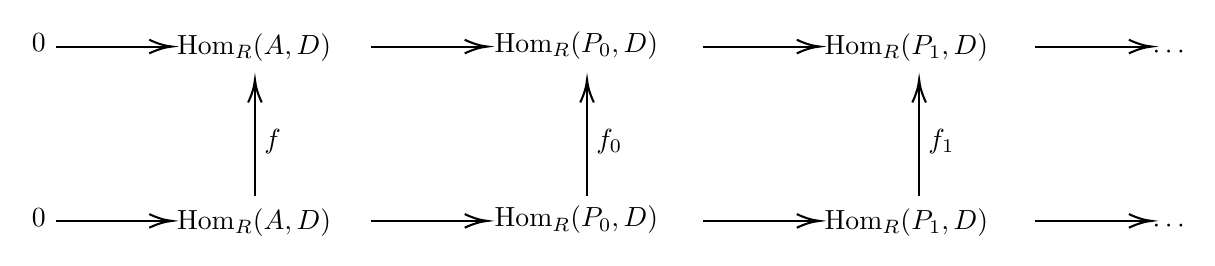
\begin{tikzpicture}[x=0.75pt,y=0.75pt,yscale=-1,xscale=1]
%uncomment if require: \path (0,476); %set diagram left start at 0, and has height of 476

%Straight Lines [id:da8448734009323151] 
\draw    (56,128) -- (110,128) ;
\draw [shift={(112,128)}, rotate = 180] [color={rgb, 255:red, 0; green, 0; blue, 0 }  ][line width=0.75]    (10.93,-3.29) .. controls (6.95,-1.4) and (3.31,-0.3) .. (0,0) .. controls (3.31,0.3) and (6.95,1.4) .. (10.93,3.29)   ;
%Straight Lines [id:da6541021433435694] 
\draw    (208,128) -- (262,128) ;
\draw [shift={(264,128)}, rotate = 180] [color={rgb, 255:red, 0; green, 0; blue, 0 }  ][line width=0.75]    (10.93,-3.29) .. controls (6.95,-1.4) and (3.31,-0.3) .. (0,0) .. controls (3.31,0.3) and (6.95,1.4) .. (10.93,3.29)   ;
%Straight Lines [id:da7793006241207661] 
\draw    (368,128) -- (422,128) ;
\draw [shift={(424,128)}, rotate = 180] [color={rgb, 255:red, 0; green, 0; blue, 0 }  ][line width=0.75]    (10.93,-3.29) .. controls (6.95,-1.4) and (3.31,-0.3) .. (0,0) .. controls (3.31,0.3) and (6.95,1.4) .. (10.93,3.29)   ;
%Straight Lines [id:da2733436751454281] 
\draw    (528,128) -- (582,128) ;
\draw [shift={(584,128)}, rotate = 180] [color={rgb, 255:red, 0; green, 0; blue, 0 }  ][line width=0.75]    (10.93,-3.29) .. controls (6.95,-1.4) and (3.31,-0.3) .. (0,0) .. controls (3.31,0.3) and (6.95,1.4) .. (10.93,3.29)   ;
%Straight Lines [id:da09185027202029672] 
\draw    (56,212) -- (110,212) ;
\draw [shift={(112,212)}, rotate = 180] [color={rgb, 255:red, 0; green, 0; blue, 0 }  ][line width=0.75]    (10.93,-3.29) .. controls (6.95,-1.4) and (3.31,-0.3) .. (0,0) .. controls (3.31,0.3) and (6.95,1.4) .. (10.93,3.29)   ;
%Straight Lines [id:da021148271926506146] 
\draw    (208,212) -- (262,212) ;
\draw [shift={(264,212)}, rotate = 180] [color={rgb, 255:red, 0; green, 0; blue, 0 }  ][line width=0.75]    (10.93,-3.29) .. controls (6.95,-1.4) and (3.31,-0.3) .. (0,0) .. controls (3.31,0.3) and (6.95,1.4) .. (10.93,3.29)   ;
%Straight Lines [id:da3810052216922586] 
\draw    (368,212) -- (422,212) ;
\draw [shift={(424,212)}, rotate = 180] [color={rgb, 255:red, 0; green, 0; blue, 0 }  ][line width=0.75]    (10.93,-3.29) .. controls (6.95,-1.4) and (3.31,-0.3) .. (0,0) .. controls (3.31,0.3) and (6.95,1.4) .. (10.93,3.29)   ;
%Straight Lines [id:da8012519674350427] 
\draw    (528,212) -- (582,212) ;
\draw [shift={(584,212)}, rotate = 180] [color={rgb, 255:red, 0; green, 0; blue, 0 }  ][line width=0.75]    (10.93,-3.29) .. controls (6.95,-1.4) and (3.31,-0.3) .. (0,0) .. controls (3.31,0.3) and (6.95,1.4) .. (10.93,3.29)   ;
%Straight Lines [id:da7160119591486331] 
\draw    (152,200) -- (152,146) ;
\draw [shift={(152,144)}, rotate = 90] [color={rgb, 255:red, 0; green, 0; blue, 0 }  ][line width=0.75]    (10.93,-3.29) .. controls (6.95,-1.4) and (3.31,-0.3) .. (0,0) .. controls (3.31,0.3) and (6.95,1.4) .. (10.93,3.29)   ;
%Straight Lines [id:da8882122178734106] 
\draw    (312,200) -- (312,146) ;
\draw [shift={(312,144)}, rotate = 90] [color={rgb, 255:red, 0; green, 0; blue, 0 }  ][line width=0.75]    (10.93,-3.29) .. controls (6.95,-1.4) and (3.31,-0.3) .. (0,0) .. controls (3.31,0.3) and (6.95,1.4) .. (10.93,3.29)   ;
%Straight Lines [id:da24042638214813938] 
\draw    (472,200) -- (472,146) ;
\draw [shift={(472,144)}, rotate = 90] [color={rgb, 255:red, 0; green, 0; blue, 0 }  ][line width=0.75]    (10.93,-3.29) .. controls (6.95,-1.4) and (3.31,-0.3) .. (0,0) .. controls (3.31,0.3) and (6.95,1.4) .. (10.93,3.29)   ;

% Text Node
\draw (43,120.4) node [anchor=north west][inner sep=0.75pt]    {$0$};
% Text Node
\draw (113,120.4) node [anchor=north west][inner sep=0.75pt]    {$\mathrm{Hom}_{R}( A,D)$};
% Text Node
\draw (266,119.4) node [anchor=north west][inner sep=0.75pt]    {$\mathrm{Hom}_{R}( P_{0} ,D)$};
% Text Node
\draw (425,120.4) node [anchor=north west][inner sep=0.75pt]    {$\mathrm{Hom}_{R}( P_{1} ,D)$};
% Text Node
\draw (43,204.4) node [anchor=north west][inner sep=0.75pt]    {$0$};
% Text Node
\draw (113,204.4) node [anchor=north west][inner sep=0.75pt]    {$\mathrm{Hom}_{R}( A,D)$};
% Text Node
\draw (266,203.4) node [anchor=north west][inner sep=0.75pt]    {$\mathrm{Hom}_{R}( P_{0} ,D)$};
% Text Node
\draw (425,204.4) node [anchor=north west][inner sep=0.75pt]    {$\mathrm{Hom}_{R}( P_{1} ,D)$};
% Text Node
\draw (155,166.4) node [anchor=north west][inner sep=0.75pt]    {$f$};
% Text Node
\draw (315,166.4) node [anchor=north west][inner sep=0.75pt]    {$f_{0}$};
% Text Node
\draw (475,166.4) node [anchor=north west][inner sep=0.75pt]    {$f_{1}$};
% Text Node
\draw (583,126.4) node [anchor=north west][inner sep=0.75pt]    {$\cdots $};
% Text Node
\draw (583,210.4) node [anchor=north west][inner sep=0.75pt]    {$\cdots $};


\end{tikzpicture}
\end{center}
is also commutative. The two rows of this diagram are cochain complexes, and this commutative diagram depicts a homomorphism of these cochain complexes. The following proposition gives an induced map on their cohomology groups.
\begin{proposition}
Let $f:A\to A^\prime$ be a homomorphism of $R$-modules and take projective resolutions of $A$ and $A^\prime$ as in Proposition A.8. Then for every $n$ there is an induced map $\varphi_n:\mathrm{Ext}_R^n(A^\prime,D)\to\mathrm{Ext}_R^n(A,D)$ on the cohomology groups obtained via these resolutions, and the maps $\varphi_n$ depend only on $f$.
\end{proposition}
\begin{proof}
The existence of such $\varphi_n$ are easy. The more difficult part is to show that they are independent of the choice of $f_n$. It suffices to show that if $f$ is the zero map, then the induced maps on cohomology groups are also zero. Assume that $f=0$, by the projectivity of the modules $P_i$ one may inductively define $R$-module homomorphisms $s_n:P_n\to P_{n+1}^\prime$ with the property that for all $n$, we have $f_n=d_{n+1}^\prime s_n+s_{n-1}d_n$, so the maps $s_n$ give reverse downward diagonal arrows across the squares: 
\begin{center}


\tikzset{every picture/.style={line width=0.75pt}} %set default line width to 0.75pt        

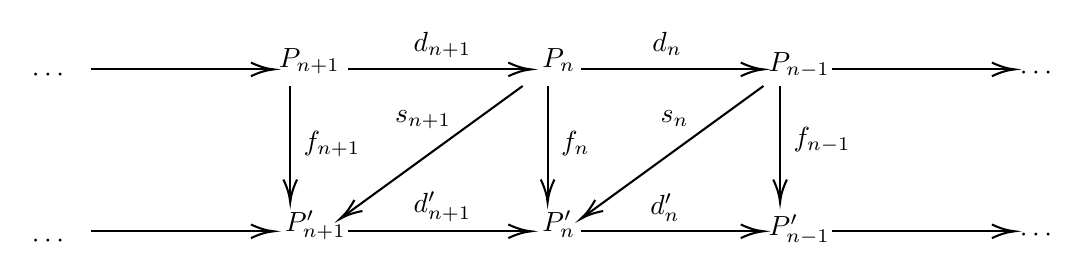
\begin{tikzpicture}[x=0.75pt,y=0.75pt,yscale=-1,xscale=1]
%uncomment if require: \path (0,476); %set diagram left start at 0, and has height of 476

%Straight Lines [id:da8460483192008399] 
\draw    (136,144) -- (222,144) ;
\draw [shift={(224,144)}, rotate = 180] [color={rgb, 255:red, 0; green, 0; blue, 0 }  ][line width=0.75]    (10.93,-3.29) .. controls (6.95,-1.4) and (3.31,-0.3) .. (0,0) .. controls (3.31,0.3) and (6.95,1.4) .. (10.93,3.29)   ;
%Straight Lines [id:da015769832717114296] 
\draw    (260,144) -- (346,144) ;
\draw [shift={(348,144)}, rotate = 180] [color={rgb, 255:red, 0; green, 0; blue, 0 }  ][line width=0.75]    (10.93,-3.29) .. controls (6.95,-1.4) and (3.31,-0.3) .. (0,0) .. controls (3.31,0.3) and (6.95,1.4) .. (10.93,3.29)   ;
%Straight Lines [id:da5890593660239558] 
\draw    (372,144) -- (458,144) ;
\draw [shift={(460,144)}, rotate = 180] [color={rgb, 255:red, 0; green, 0; blue, 0 }  ][line width=0.75]    (10.93,-3.29) .. controls (6.95,-1.4) and (3.31,-0.3) .. (0,0) .. controls (3.31,0.3) and (6.95,1.4) .. (10.93,3.29)   ;
%Straight Lines [id:da4893697163001278] 
\draw    (493,144) -- (579,144) ;
\draw [shift={(581,144)}, rotate = 180] [color={rgb, 255:red, 0; green, 0; blue, 0 }  ][line width=0.75]    (10.93,-3.29) .. controls (6.95,-1.4) and (3.31,-0.3) .. (0,0) .. controls (3.31,0.3) and (6.95,1.4) .. (10.93,3.29)   ;
%Straight Lines [id:da16530627275642962] 
\draw    (136,222) -- (222,222) ;
\draw [shift={(224,222)}, rotate = 180] [color={rgb, 255:red, 0; green, 0; blue, 0 }  ][line width=0.75]    (10.93,-3.29) .. controls (6.95,-1.4) and (3.31,-0.3) .. (0,0) .. controls (3.31,0.3) and (6.95,1.4) .. (10.93,3.29)   ;
%Straight Lines [id:da35122803984286666] 
\draw    (260,222) -- (346,222) ;
\draw [shift={(348,222)}, rotate = 180] [color={rgb, 255:red, 0; green, 0; blue, 0 }  ][line width=0.75]    (10.93,-3.29) .. controls (6.95,-1.4) and (3.31,-0.3) .. (0,0) .. controls (3.31,0.3) and (6.95,1.4) .. (10.93,3.29)   ;
%Straight Lines [id:da27326836730802095] 
\draw    (372,222) -- (458,222) ;
\draw [shift={(460,222)}, rotate = 180] [color={rgb, 255:red, 0; green, 0; blue, 0 }  ][line width=0.75]    (10.93,-3.29) .. controls (6.95,-1.4) and (3.31,-0.3) .. (0,0) .. controls (3.31,0.3) and (6.95,1.4) .. (10.93,3.29)   ;
%Straight Lines [id:da5307504663973357] 
\draw    (493,222) -- (579,222) ;
\draw [shift={(581,222)}, rotate = 180] [color={rgb, 255:red, 0; green, 0; blue, 0 }  ][line width=0.75]    (10.93,-3.29) .. controls (6.95,-1.4) and (3.31,-0.3) .. (0,0) .. controls (3.31,0.3) and (6.95,1.4) .. (10.93,3.29)   ;
%Straight Lines [id:da7525902918596272] 
\draw    (232,152) -- (232,206) ;
\draw [shift={(232,208)}, rotate = 270] [color={rgb, 255:red, 0; green, 0; blue, 0 }  ][line width=0.75]    (10.93,-3.29) .. controls (6.95,-1.4) and (3.31,-0.3) .. (0,0) .. controls (3.31,0.3) and (6.95,1.4) .. (10.93,3.29)   ;
%Straight Lines [id:da9644455390597471] 
\draw    (356,152) -- (356,206) ;
\draw [shift={(356,208)}, rotate = 270] [color={rgb, 255:red, 0; green, 0; blue, 0 }  ][line width=0.75]    (10.93,-3.29) .. controls (6.95,-1.4) and (3.31,-0.3) .. (0,0) .. controls (3.31,0.3) and (6.95,1.4) .. (10.93,3.29)   ;
%Straight Lines [id:da7230033607989828] 
\draw    (468,152) -- (468,206) ;
\draw [shift={(468,208)}, rotate = 270] [color={rgb, 255:red, 0; green, 0; blue, 0 }  ][line width=0.75]    (10.93,-3.29) .. controls (6.95,-1.4) and (3.31,-0.3) .. (0,0) .. controls (3.31,0.3) and (6.95,1.4) .. (10.93,3.29)   ;
%Straight Lines [id:da34049584882200135] 
\draw    (344,152) -- (257.62,214.82) ;
\draw [shift={(256,216)}, rotate = 323.97] [color={rgb, 255:red, 0; green, 0; blue, 0 }  ][line width=0.75]    (10.93,-3.29) .. controls (6.95,-1.4) and (3.31,-0.3) .. (0,0) .. controls (3.31,0.3) and (6.95,1.4) .. (10.93,3.29)   ;
%Straight Lines [id:da14933210259162344] 
\draw    (460,152) -- (373.62,214.82) ;
\draw [shift={(372,216)}, rotate = 323.97] [color={rgb, 255:red, 0; green, 0; blue, 0 }  ][line width=0.75]    (10.93,-3.29) .. controls (6.95,-1.4) and (3.31,-0.3) .. (0,0) .. controls (3.31,0.3) and (6.95,1.4) .. (10.93,3.29)   ;

% Text Node
\draw (225,132.4) node [anchor=north west][inner sep=0.75pt]    {$P_{n+1}$};
% Text Node
\draw (352,132.4) node [anchor=north west][inner sep=0.75pt]    {$P_{n}$};
% Text Node
\draw (461,134.4) node [anchor=north west][inner sep=0.75pt]    {$P_{n-1}$};
% Text Node
\draw (582,141.4) node [anchor=north west][inner sep=0.75pt]    {$\cdots $};
% Text Node
\draw (228,210.4) node [anchor=north west][inner sep=0.75pt]    {$P_{n+1}^{\prime }$};
% Text Node
\draw (352,210.4) node [anchor=north west][inner sep=0.75pt]    {$P_{n}^{\prime }$};
% Text Node
\draw (461,212.4) node [anchor=north west][inner sep=0.75pt]    {$P_{n-1}^{\prime }$};
% Text Node
\draw (582,219.4) node [anchor=north west][inner sep=0.75pt]    {$\cdots $};
% Text Node
\draw (106,142.4) node [anchor=north west][inner sep=0.75pt]    {$\cdots $};
% Text Node
\draw (106,222.4) node [anchor=north west][inner sep=0.75pt]    {$\cdots $};
% Text Node
\draw (290,124.4) node [anchor=north west][inner sep=0.75pt]    {$d_{n+1}$};
% Text Node
\draw (405,124.4) node [anchor=north west][inner sep=0.75pt]    {$d_{n}$};
% Text Node
\draw (290,201.4) node [anchor=north west][inner sep=0.75pt]    {$d_{n+1}^{\prime }$};
% Text Node
\draw (404,202.4) node [anchor=north west][inner sep=0.75pt]    {$d_{n}^{\prime }$};
% Text Node
\draw (237,172.4) node [anchor=north west][inner sep=0.75pt]    {$f_{n+1}$};
% Text Node
\draw (361,172.4) node [anchor=north west][inner sep=0.75pt]    {$f_{n}$};
% Text Node
\draw (473,170.4) node [anchor=north west][inner sep=0.75pt]    {$f_{n-1}$};
% Text Node
\draw (281,162.4) node [anchor=north west][inner sep=0.75pt]    {$s_{n+1}$};
% Text Node
\draw (409,162.4) node [anchor=north west][inner sep=0.75pt]    {$s_{n}$};


\end{tikzpicture}
\end{center}
Taking homomorphisms into $D$ gives the following commutative diagram: 
\begin{figure}[htbp]
    \center
    \includegraphics[scale=0.29]{Images/diagram-20240314 (2).png}
\end{figure}
It is now easy to see that any element in $\mathrm{Hom}_R(P_n^\prime,D)$ representing a coset in $\mathrm{Ext}_R^n(A^\prime,D)$ maps to the zero coset in $\mathrm{Ext}_R^n(A,D)$. This completes the argument.
\end{proof}
With these propositions, we may proof the following theorem.
\begin{theorem}
The groups $\mathrm{Ext}_R^n(A,D)$ depend only on $A$ and $D$, i.e. they are independent of the choice of projective resolution of $A$.
\end{theorem}
\begin{proof}
We adopt the preceding notations. Let $A^\prime=A$, $f:A\to A^\prime$ the identity map. Consider the following diagram: 
\begin{center}


\tikzset{every picture/.style={line width=0.75pt}} %set default line width to 0.75pt        

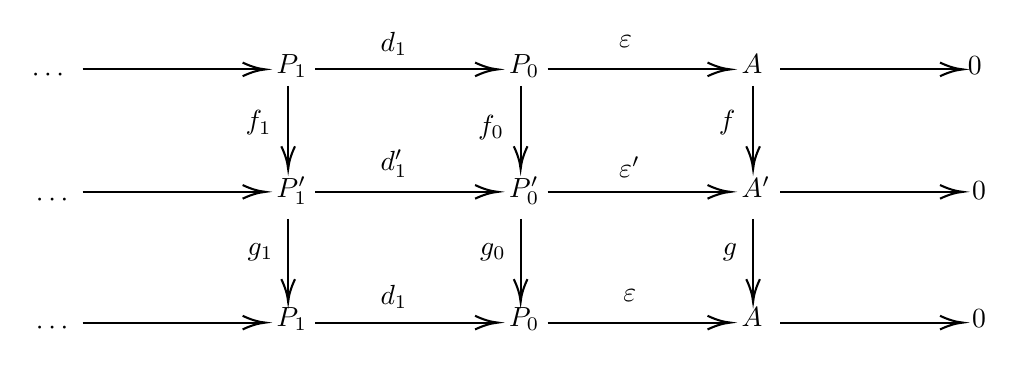
\begin{tikzpicture}[x=0.75pt,y=0.75pt,yscale=-1,xscale=1]
%uncomment if require: \path (0,476); %set diagram left start at 0, and has height of 476

%Straight Lines [id:da44711984370424007] 
\draw    (120,144) -- (206,144) ;
\draw [shift={(208,144)}, rotate = 180] [color={rgb, 255:red, 0; green, 0; blue, 0 }  ][line width=0.75]    (10.93,-3.29) .. controls (6.95,-1.4) and (3.31,-0.3) .. (0,0) .. controls (3.31,0.3) and (6.95,1.4) .. (10.93,3.29)   ;
%Straight Lines [id:da9248725977596619] 
\draw    (232,144) -- (318,144) ;
\draw [shift={(320,144)}, rotate = 180] [color={rgb, 255:red, 0; green, 0; blue, 0 }  ][line width=0.75]    (10.93,-3.29) .. controls (6.95,-1.4) and (3.31,-0.3) .. (0,0) .. controls (3.31,0.3) and (6.95,1.4) .. (10.93,3.29)   ;
%Straight Lines [id:da6138692033765099] 
\draw    (344,144) -- (430,144) ;
\draw [shift={(432,144)}, rotate = 180] [color={rgb, 255:red, 0; green, 0; blue, 0 }  ][line width=0.75]    (10.93,-3.29) .. controls (6.95,-1.4) and (3.31,-0.3) .. (0,0) .. controls (3.31,0.3) and (6.95,1.4) .. (10.93,3.29)   ;
%Straight Lines [id:da987248452532802] 
\draw    (456,144) -- (542,144) ;
\draw [shift={(544,144)}, rotate = 180] [color={rgb, 255:red, 0; green, 0; blue, 0 }  ][line width=0.75]    (10.93,-3.29) .. controls (6.95,-1.4) and (3.31,-0.3) .. (0,0) .. controls (3.31,0.3) and (6.95,1.4) .. (10.93,3.29)   ;
%Straight Lines [id:da6220099634108145] 
\draw    (120,203) -- (206,203) ;
\draw [shift={(208,203)}, rotate = 180] [color={rgb, 255:red, 0; green, 0; blue, 0 }  ][line width=0.75]    (10.93,-3.29) .. controls (6.95,-1.4) and (3.31,-0.3) .. (0,0) .. controls (3.31,0.3) and (6.95,1.4) .. (10.93,3.29)   ;
%Straight Lines [id:da29136558382735456] 
\draw    (232,203) -- (318,203) ;
\draw [shift={(320,203)}, rotate = 180] [color={rgb, 255:red, 0; green, 0; blue, 0 }  ][line width=0.75]    (10.93,-3.29) .. controls (6.95,-1.4) and (3.31,-0.3) .. (0,0) .. controls (3.31,0.3) and (6.95,1.4) .. (10.93,3.29)   ;
%Straight Lines [id:da13231241165652796] 
\draw    (344,203) -- (430,203) ;
\draw [shift={(432,203)}, rotate = 180] [color={rgb, 255:red, 0; green, 0; blue, 0 }  ][line width=0.75]    (10.93,-3.29) .. controls (6.95,-1.4) and (3.31,-0.3) .. (0,0) .. controls (3.31,0.3) and (6.95,1.4) .. (10.93,3.29)   ;
%Straight Lines [id:da42865383949106994] 
\draw    (456,203) -- (542,203) ;
\draw [shift={(544,203)}, rotate = 180] [color={rgb, 255:red, 0; green, 0; blue, 0 }  ][line width=0.75]    (10.93,-3.29) .. controls (6.95,-1.4) and (3.31,-0.3) .. (0,0) .. controls (3.31,0.3) and (6.95,1.4) .. (10.93,3.29)   ;
%Straight Lines [id:da45701835500395505] 
\draw    (120,266) -- (206,266) ;
\draw [shift={(208,266)}, rotate = 180] [color={rgb, 255:red, 0; green, 0; blue, 0 }  ][line width=0.75]    (10.93,-3.29) .. controls (6.95,-1.4) and (3.31,-0.3) .. (0,0) .. controls (3.31,0.3) and (6.95,1.4) .. (10.93,3.29)   ;
%Straight Lines [id:da3539691933000293] 
\draw    (232,266) -- (318,266) ;
\draw [shift={(320,266)}, rotate = 180] [color={rgb, 255:red, 0; green, 0; blue, 0 }  ][line width=0.75]    (10.93,-3.29) .. controls (6.95,-1.4) and (3.31,-0.3) .. (0,0) .. controls (3.31,0.3) and (6.95,1.4) .. (10.93,3.29)   ;
%Straight Lines [id:da580572215263433] 
\draw    (344,266) -- (430,266) ;
\draw [shift={(432,266)}, rotate = 180] [color={rgb, 255:red, 0; green, 0; blue, 0 }  ][line width=0.75]    (10.93,-3.29) .. controls (6.95,-1.4) and (3.31,-0.3) .. (0,0) .. controls (3.31,0.3) and (6.95,1.4) .. (10.93,3.29)   ;
%Straight Lines [id:da7004280674500418] 
\draw    (456,266) -- (542,266) ;
\draw [shift={(544,266)}, rotate = 180] [color={rgb, 255:red, 0; green, 0; blue, 0 }  ][line width=0.75]    (10.93,-3.29) .. controls (6.95,-1.4) and (3.31,-0.3) .. (0,0) .. controls (3.31,0.3) and (6.95,1.4) .. (10.93,3.29)   ;
%Straight Lines [id:da267514772226493] 
\draw    (219,152) -- (219,190) ;
\draw [shift={(219,192)}, rotate = 270] [color={rgb, 255:red, 0; green, 0; blue, 0 }  ][line width=0.75]    (10.93,-3.29) .. controls (6.95,-1.4) and (3.31,-0.3) .. (0,0) .. controls (3.31,0.3) and (6.95,1.4) .. (10.93,3.29)   ;
%Straight Lines [id:da9727672287325093] 
\draw    (331,152) -- (331,190) ;
\draw [shift={(331,192)}, rotate = 270] [color={rgb, 255:red, 0; green, 0; blue, 0 }  ][line width=0.75]    (10.93,-3.29) .. controls (6.95,-1.4) and (3.31,-0.3) .. (0,0) .. controls (3.31,0.3) and (6.95,1.4) .. (10.93,3.29)   ;
%Straight Lines [id:da7780388414096724] 
\draw    (443,152) -- (443,190) ;
\draw [shift={(443,192)}, rotate = 270] [color={rgb, 255:red, 0; green, 0; blue, 0 }  ][line width=0.75]    (10.93,-3.29) .. controls (6.95,-1.4) and (3.31,-0.3) .. (0,0) .. controls (3.31,0.3) and (6.95,1.4) .. (10.93,3.29)   ;
%Straight Lines [id:da46126166192329165] 
\draw    (219,216) -- (219,254) ;
\draw [shift={(219,256)}, rotate = 270] [color={rgb, 255:red, 0; green, 0; blue, 0 }  ][line width=0.75]    (10.93,-3.29) .. controls (6.95,-1.4) and (3.31,-0.3) .. (0,0) .. controls (3.31,0.3) and (6.95,1.4) .. (10.93,3.29)   ;
%Straight Lines [id:da521643270794774] 
\draw    (331,216) -- (331,254) ;
\draw [shift={(331,256)}, rotate = 270] [color={rgb, 255:red, 0; green, 0; blue, 0 }  ][line width=0.75]    (10.93,-3.29) .. controls (6.95,-1.4) and (3.31,-0.3) .. (0,0) .. controls (3.31,0.3) and (6.95,1.4) .. (10.93,3.29)   ;
%Straight Lines [id:da3031582407175466] 
\draw    (443,216) -- (443,254) ;
\draw [shift={(443,256)}, rotate = 270] [color={rgb, 255:red, 0; green, 0; blue, 0 }  ][line width=0.75]    (10.93,-3.29) .. controls (6.95,-1.4) and (3.31,-0.3) .. (0,0) .. controls (3.31,0.3) and (6.95,1.4) .. (10.93,3.29)   ;

% Text Node
\draw (212,135.4) node [anchor=north west][inner sep=0.75pt]    {$P_{1}$};
% Text Node
\draw (324,135.4) node [anchor=north west][inner sep=0.75pt]    {$P_{0}$};
% Text Node
\draw (436,135.4) node [anchor=north west][inner sep=0.75pt]    {$A$};
% Text Node
\draw (212,194.4) node [anchor=north west][inner sep=0.75pt]    {$P_{1}^{\prime }$};
% Text Node
\draw (324,194.4) node [anchor=north west][inner sep=0.75pt]    {$P_{0}^{\prime }$};
% Text Node
\draw (436,194.4) node [anchor=north west][inner sep=0.75pt]    {$A^{\prime }$};
% Text Node
\draw (212,257.4) node [anchor=north west][inner sep=0.75pt]    {$P_{1}$};
% Text Node
\draw (324,257.4) node [anchor=north west][inner sep=0.75pt]    {$P_{0}$};
% Text Node
\draw (436,257.4) node [anchor=north west][inner sep=0.75pt]    {$A$};
% Text Node
\draw (262,124.4) node [anchor=north west][inner sep=0.75pt]    {$d_{1}$};
% Text Node
\draw (262,181.4) node [anchor=north west][inner sep=0.75pt]    {$d_{1}^{\prime }$};
% Text Node
\draw (262,246.4) node [anchor=north west][inner sep=0.75pt]    {$d_{1}$};
% Text Node
\draw (377,126.4) node [anchor=north west][inner sep=0.75pt]    {$\varepsilon $};
% Text Node
\draw (377,184.4) node [anchor=north west][inner sep=0.75pt]    {$\varepsilon ^{\prime }$};
% Text Node
\draw (379,248.4) node [anchor=north west][inner sep=0.75pt]    {$\varepsilon $};
% Text Node
\draw (545,136.4) node [anchor=north west][inner sep=0.75pt]    {$0$};
% Text Node
\draw (547,196.4) node [anchor=north west][inner sep=0.75pt]    {$0$};
% Text Node
\draw (547,258.4) node [anchor=north west][inner sep=0.75pt]    {$0$};
% Text Node
\draw (94,142.4) node [anchor=north west][inner sep=0.75pt]    {$\cdots $};
% Text Node
\draw (96,202.4) node [anchor=north west][inner sep=0.75pt]    {$\cdots $};
% Text Node
\draw (96,264.4) node [anchor=north west][inner sep=0.75pt]    {$\cdots $};
% Text Node
\draw (197,162.4) node [anchor=north west][inner sep=0.75pt]    {$f_{1}$};
% Text Node
\draw (309,164.4) node [anchor=north west][inner sep=0.75pt]    {$f_{0}$};
% Text Node
\draw (425,162.4) node [anchor=north west][inner sep=0.75pt]    {$f$};
% Text Node
\draw (427,226.4) node [anchor=north west][inner sep=0.75pt]    {$g$};
% Text Node
\draw (198,226.4) node [anchor=north west][inner sep=0.75pt]    {$g_{1}$};
% Text Node
\draw (310,226.4) node [anchor=north west][inner sep=0.75pt]    {$g_{0}$};


\end{tikzpicture}
\end{center}
where $g$ is the identity map from $A^\prime$ to $A$. Let $\varphi_n$ and $\psi_n$ be the induced maps on the cohomology groups of the first and last two rows. Now the map $g_n\circ f_n$ are a lift of the identity map $g\circ f$, and hence they induce the homomorphisms $\varphi_n\circ\psi_n$ on the cohomology groups. However the first and the third row are identical, this implies $\varphi_i\circ\psi_n$ is also the identity on $\mathrm{Ext}_R^n(A,D)$. By a symmetric argument we have similar results on $\psi\circ\varphi$, which finished the proof.
\end{proof}
We now turn to some basic properties of the $\mathrm{Ext}$ functor.
\begin{proposition}{\textbf{(Simultaneous Resolution)}}
Let 
$$
0\longrightarrow L\longrightarrow M\longrightarrow N\longrightarrow 0
$$
be a short exact sequence of $R$-modules. Suppose 
$$
\cdots \longrightarrow P_1\longrightarrow P_0\longrightarrow L\longrightarrow 0
$$
and 
$$
\cdots \longrightarrow \overline{P_1}\longrightarrow \overline{P_0}\longrightarrow N\longrightarrow 0
$$
are both projective resolutions. Then there is a resolution of $M$ by the projective modules $P_n\oplus\overline{P_n}$ such that the following diagram commutes: 
\begin{center}


\tikzset{every picture/.style={line width=0.75pt}} %set default line width to 0.75pt        

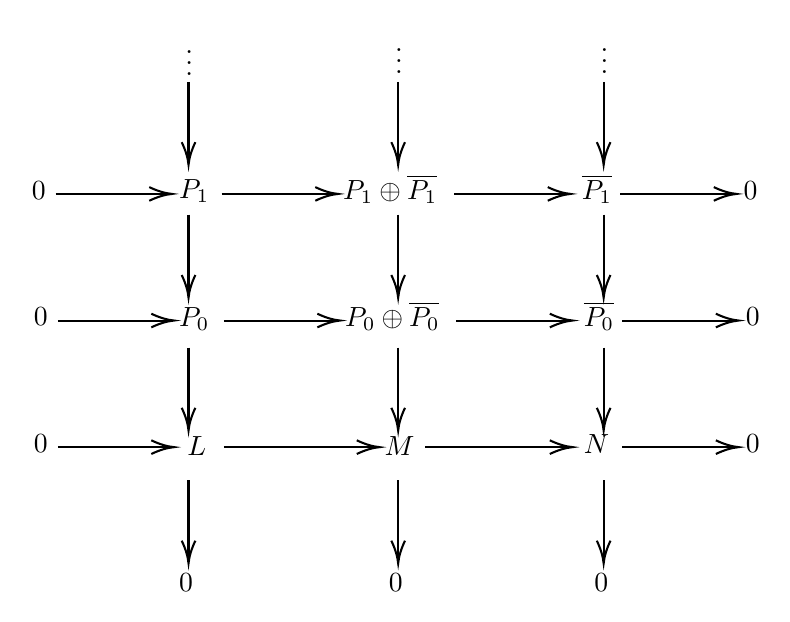
\begin{tikzpicture}[x=0.75pt,y=0.75pt,yscale=-1,xscale=1]
%uncomment if require: \path (0,476); %set diagram left start at 0, and has height of 476

%Straight Lines [id:da25780887338366676] 
\draw    (144,110) -- (198,110) ;
\draw [shift={(200,110)}, rotate = 180] [color={rgb, 255:red, 0; green, 0; blue, 0 }  ][line width=0.75]    (10.93,-3.29) .. controls (6.95,-1.4) and (3.31,-0.3) .. (0,0) .. controls (3.31,0.3) and (6.95,1.4) .. (10.93,3.29)   ;
%Straight Lines [id:da2296304050834892] 
\draw    (224,110) -- (278,110) ;
\draw [shift={(280,110)}, rotate = 180] [color={rgb, 255:red, 0; green, 0; blue, 0 }  ][line width=0.75]    (10.93,-3.29) .. controls (6.95,-1.4) and (3.31,-0.3) .. (0,0) .. controls (3.31,0.3) and (6.95,1.4) .. (10.93,3.29)   ;
%Straight Lines [id:da13701935238363117] 
\draw    (336,110) -- (390,110) ;
\draw [shift={(392,110)}, rotate = 180] [color={rgb, 255:red, 0; green, 0; blue, 0 }  ][line width=0.75]    (10.93,-3.29) .. controls (6.95,-1.4) and (3.31,-0.3) .. (0,0) .. controls (3.31,0.3) and (6.95,1.4) .. (10.93,3.29)   ;
%Straight Lines [id:da2808655717202371] 
\draw    (416,110) -- (470,110) ;
\draw [shift={(472,110)}, rotate = 180] [color={rgb, 255:red, 0; green, 0; blue, 0 }  ][line width=0.75]    (10.93,-3.29) .. controls (6.95,-1.4) and (3.31,-0.3) .. (0,0) .. controls (3.31,0.3) and (6.95,1.4) .. (10.93,3.29)   ;
%Straight Lines [id:da22913437966437744] 
\draw    (145,171) -- (199,171) ;
\draw [shift={(201,171)}, rotate = 180] [color={rgb, 255:red, 0; green, 0; blue, 0 }  ][line width=0.75]    (10.93,-3.29) .. controls (6.95,-1.4) and (3.31,-0.3) .. (0,0) .. controls (3.31,0.3) and (6.95,1.4) .. (10.93,3.29)   ;
%Straight Lines [id:da8699617542941762] 
\draw    (225,171) -- (279,171) ;
\draw [shift={(281,171)}, rotate = 180] [color={rgb, 255:red, 0; green, 0; blue, 0 }  ][line width=0.75]    (10.93,-3.29) .. controls (6.95,-1.4) and (3.31,-0.3) .. (0,0) .. controls (3.31,0.3) and (6.95,1.4) .. (10.93,3.29)   ;
%Straight Lines [id:da4535868838491668] 
\draw    (337,171) -- (391,171) ;
\draw [shift={(393,171)}, rotate = 180] [color={rgb, 255:red, 0; green, 0; blue, 0 }  ][line width=0.75]    (10.93,-3.29) .. controls (6.95,-1.4) and (3.31,-0.3) .. (0,0) .. controls (3.31,0.3) and (6.95,1.4) .. (10.93,3.29)   ;
%Straight Lines [id:da8843348365190076] 
\draw    (417,171) -- (471,171) ;
\draw [shift={(473,171)}, rotate = 180] [color={rgb, 255:red, 0; green, 0; blue, 0 }  ][line width=0.75]    (10.93,-3.29) .. controls (6.95,-1.4) and (3.31,-0.3) .. (0,0) .. controls (3.31,0.3) and (6.95,1.4) .. (10.93,3.29)   ;
%Straight Lines [id:da6477443892593087] 
\draw    (145,232) -- (199,232) ;
\draw [shift={(201,232)}, rotate = 180] [color={rgb, 255:red, 0; green, 0; blue, 0 }  ][line width=0.75]    (10.93,-3.29) .. controls (6.95,-1.4) and (3.31,-0.3) .. (0,0) .. controls (3.31,0.3) and (6.95,1.4) .. (10.93,3.29)   ;
%Straight Lines [id:da5157052669572391] 
\draw    (225,232) -- (298,232) ;
\draw [shift={(300,232)}, rotate = 180] [color={rgb, 255:red, 0; green, 0; blue, 0 }  ][line width=0.75]    (10.93,-3.29) .. controls (6.95,-1.4) and (3.31,-0.3) .. (0,0) .. controls (3.31,0.3) and (6.95,1.4) .. (10.93,3.29)   ;
%Straight Lines [id:da026266964157520167] 
\draw    (322,232) -- (391,232) ;
\draw [shift={(393,232)}, rotate = 180] [color={rgb, 255:red, 0; green, 0; blue, 0 }  ][line width=0.75]    (10.93,-3.29) .. controls (6.95,-1.4) and (3.31,-0.3) .. (0,0) .. controls (3.31,0.3) and (6.95,1.4) .. (10.93,3.29)   ;
%Straight Lines [id:da08392622041605957] 
\draw    (417,232) -- (471,232) ;
\draw [shift={(473,232)}, rotate = 180] [color={rgb, 255:red, 0; green, 0; blue, 0 }  ][line width=0.75]    (10.93,-3.29) .. controls (6.95,-1.4) and (3.31,-0.3) .. (0,0) .. controls (3.31,0.3) and (6.95,1.4) .. (10.93,3.29)   ;
%Straight Lines [id:da2044392970143285] 
\draw    (208,120) -- (208,158) ;
\draw [shift={(208,160)}, rotate = 270] [color={rgb, 255:red, 0; green, 0; blue, 0 }  ][line width=0.75]    (10.93,-3.29) .. controls (6.95,-1.4) and (3.31,-0.3) .. (0,0) .. controls (3.31,0.3) and (6.95,1.4) .. (10.93,3.29)   ;
%Straight Lines [id:da15742315833901488] 
\draw    (208,184) -- (208,222) ;
\draw [shift={(208,224)}, rotate = 270] [color={rgb, 255:red, 0; green, 0; blue, 0 }  ][line width=0.75]    (10.93,-3.29) .. controls (6.95,-1.4) and (3.31,-0.3) .. (0,0) .. controls (3.31,0.3) and (6.95,1.4) .. (10.93,3.29)   ;
%Straight Lines [id:da2428774173899848] 
\draw    (309,120) -- (309,158) ;
\draw [shift={(309,160)}, rotate = 270] [color={rgb, 255:red, 0; green, 0; blue, 0 }  ][line width=0.75]    (10.93,-3.29) .. controls (6.95,-1.4) and (3.31,-0.3) .. (0,0) .. controls (3.31,0.3) and (6.95,1.4) .. (10.93,3.29)   ;
%Straight Lines [id:da8614666682507406] 
\draw    (408,120) -- (408,158) ;
\draw [shift={(408,160)}, rotate = 270] [color={rgb, 255:red, 0; green, 0; blue, 0 }  ][line width=0.75]    (10.93,-3.29) .. controls (6.95,-1.4) and (3.31,-0.3) .. (0,0) .. controls (3.31,0.3) and (6.95,1.4) .. (10.93,3.29)   ;
%Straight Lines [id:da6581581330460078] 
\draw    (309,184) -- (309,222) ;
\draw [shift={(309,224)}, rotate = 270] [color={rgb, 255:red, 0; green, 0; blue, 0 }  ][line width=0.75]    (10.93,-3.29) .. controls (6.95,-1.4) and (3.31,-0.3) .. (0,0) .. controls (3.31,0.3) and (6.95,1.4) .. (10.93,3.29)   ;
%Straight Lines [id:da405870965174143] 
\draw    (408,184) -- (408,222) ;
\draw [shift={(408,224)}, rotate = 270] [color={rgb, 255:red, 0; green, 0; blue, 0 }  ][line width=0.75]    (10.93,-3.29) .. controls (6.95,-1.4) and (3.31,-0.3) .. (0,0) .. controls (3.31,0.3) and (6.95,1.4) .. (10.93,3.29)   ;
%Straight Lines [id:da8108655103423166] 
\draw    (208,56) -- (208,94) ;
\draw [shift={(208,96)}, rotate = 270] [color={rgb, 255:red, 0; green, 0; blue, 0 }  ][line width=0.75]    (10.93,-3.29) .. controls (6.95,-1.4) and (3.31,-0.3) .. (0,0) .. controls (3.31,0.3) and (6.95,1.4) .. (10.93,3.29)   ;
%Straight Lines [id:da00701019940599279] 
\draw    (208,248) -- (208,286) ;
\draw [shift={(208,288)}, rotate = 270] [color={rgb, 255:red, 0; green, 0; blue, 0 }  ][line width=0.75]    (10.93,-3.29) .. controls (6.95,-1.4) and (3.31,-0.3) .. (0,0) .. controls (3.31,0.3) and (6.95,1.4) .. (10.93,3.29)   ;
%Straight Lines [id:da6345022051100266] 
\draw    (408,56) -- (408,94) ;
\draw [shift={(408,96)}, rotate = 270] [color={rgb, 255:red, 0; green, 0; blue, 0 }  ][line width=0.75]    (10.93,-3.29) .. controls (6.95,-1.4) and (3.31,-0.3) .. (0,0) .. controls (3.31,0.3) and (6.95,1.4) .. (10.93,3.29)   ;
%Straight Lines [id:da38022118604164246] 
\draw    (408,248) -- (408,286) ;
\draw [shift={(408,288)}, rotate = 270] [color={rgb, 255:red, 0; green, 0; blue, 0 }  ][line width=0.75]    (10.93,-3.29) .. controls (6.95,-1.4) and (3.31,-0.3) .. (0,0) .. controls (3.31,0.3) and (6.95,1.4) .. (10.93,3.29)   ;
%Straight Lines [id:da08126891146682258] 
\draw    (309,56) -- (309,94) ;
\draw [shift={(309,96)}, rotate = 270] [color={rgb, 255:red, 0; green, 0; blue, 0 }  ][line width=0.75]    (10.93,-3.29) .. controls (6.95,-1.4) and (3.31,-0.3) .. (0,0) .. controls (3.31,0.3) and (6.95,1.4) .. (10.93,3.29)   ;
%Straight Lines [id:da4850345796340001] 
\draw    (309,248) -- (309,286) ;
\draw [shift={(309,288)}, rotate = 270] [color={rgb, 255:red, 0; green, 0; blue, 0 }  ][line width=0.75]    (10.93,-3.29) .. controls (6.95,-1.4) and (3.31,-0.3) .. (0,0) .. controls (3.31,0.3) and (6.95,1.4) .. (10.93,3.29)   ;

% Text Node
\draw (131,102.4) node [anchor=north west][inner sep=0.75pt]    {$0$};
% Text Node
\draw (202,101.4) node [anchor=north west][inner sep=0.75pt]    {$P_{1}$};
% Text Node
\draw (281,99.4) node [anchor=north west][inner sep=0.75pt]    {$P_{1} \oplus \overline{P_{1}}$};
% Text Node
\draw (396,99.4) node [anchor=north west][inner sep=0.75pt]    {$\overline{P_{1}}$};
% Text Node
\draw (474,102.4) node [anchor=north west][inner sep=0.75pt]    {$0$};
% Text Node
\draw (132,163.4) node [anchor=north west][inner sep=0.75pt]    {$0$};
% Text Node
\draw (202,163.4) node [anchor=north west][inner sep=0.75pt]    {$P_{0}$};
% Text Node
\draw (282,160.4) node [anchor=north west][inner sep=0.75pt]    {$P_{0} \oplus \overline{P_{0}}$};
% Text Node
\draw (397,160.4) node [anchor=north west][inner sep=0.75pt]    {$\overline{P_{0}}$};
% Text Node
\draw (475,163.4) node [anchor=north west][inner sep=0.75pt]    {$0$};
% Text Node
\draw (132,224.4) node [anchor=north west][inner sep=0.75pt]    {$0$};
% Text Node
\draw (206,225.4) node [anchor=north west][inner sep=0.75pt]    {$L$};
% Text Node
\draw (301,225.4) node [anchor=north west][inner sep=0.75pt]    {$M$};
% Text Node
\draw (397,224.4) node [anchor=north west][inner sep=0.75pt]    {$N$};
% Text Node
\draw (475,224.4) node [anchor=north west][inner sep=0.75pt]    {$0$};
% Text Node
\draw (202,291.4) node [anchor=north west][inner sep=0.75pt]    {$0$};
% Text Node
\draw (303,291.4) node [anchor=north west][inner sep=0.75pt]    {$0$};
% Text Node
\draw (402,291.4) node [anchor=north west][inner sep=0.75pt]    {$0$};
% Text Node
\draw (205,31.4) node [anchor=north west][inner sep=0.75pt]    {$\vdots $};
% Text Node
\draw (306,30.4) node [anchor=north west][inner sep=0.75pt]    {$\vdots $};
% Text Node
\draw (405,30.4) node [anchor=north west][inner sep=0.75pt]    {$\vdots $};


\end{tikzpicture}
\end{center}
Moreover, the rows and columns of this diagram are exact ans the rows are split.
\end{proposition}
\begin{proof}
Since $P_i$ and $\overline{P_i}$ are both projective $R$-modules, it follows immediately that $P_i\oplus\overline{P_i}$ is also a projective $R$-module. Therefore the middle column is a projective resolution. To show the diagram commutes, it suffices to define the maps $P_i\oplus\overline{P_i}$ properly. By the lifting property of a projective module, we may define $\mu:\overline{P_0}\to M$. Define also $\lambda:P_0\to M$ by the composition of maps, then define $\pi_0:P_0\oplus\overline{P_0}\to M$ by $(x,y)\mapsto\mu(x)+\lambda(y)$. Define inductively and it is routine to check the diagram is commutative.
\end{proof}
\begin{theorem}
Let 
$$
0\longrightarrow L\longrightarrow M\longrightarrow N\longrightarrow 0
$$
be a short exact sequence. Then there exists a long exact sequence 
$$
0\longrightarrow \mathrm{Hom}_R\left( N,D \right) \longrightarrow \mathrm{Hom}_R\left( M,D \right) \longrightarrow \mathrm{Hom}_R\left( L,D \right) \longrightarrow \mathrm{Ext}_{R}^{1}\left( N,D \right) \longrightarrow \cdots ,
$$
where the homomorphisms are defined as in Theorem A.4.
\end{theorem}
\begin{proof}
By Theorem A.4 it suffices to show that there are a series of short exact sequences 
$$
0\longrightarrow \mathrm{Hom}_R\left( \overline{P_i},D \right) \longrightarrow \mathrm{Hom}_R\left( \overline{P_i}\oplus P_i,D \right) \longrightarrow \mathrm{Hom}_R\left( P_i,D \right) \longrightarrow 0,
$$
then by Theorem A.4 the proof is finished. Note that this follows from the simultaneous resolution: \par
\begin{figure}[htbp]
    \center
    \includegraphics[scale=0.24]{Images/diagram-20240314 (4).png}
\end{figure}
which finished the proof.
\end{proof}
By Theorem A.12 we may obtain a characterization of projective and injective modules.
\begin{theorem}
For any $R$-module $P$ we have the following equivalent conditions: \par
(i) $P$ is a projective module.\par
(ii) $\mathrm{Ext}_R^1(P,D)=0$ for any $R$-module $D$.\par
(iii) $\mathrm{Ext}_R^n(P,D)=0$ for any $R$-module $D$.
\end{theorem}
\begin{proof}
(iii)$\Rightarrow$(ii): Trivial.\par
(ii)$\Rightarrow$(i): Suppose $\mathrm{Ext}_R^1(P,D)=0$ for all $R$-module $D$, then we have 
$$
0\longrightarrow \mathrm{Hom}_R\left( P,N \right) \longrightarrow \mathrm{Hom}_R\left( P,M \right) \longrightarrow \mathrm{Hom}_R\left( P,L \right) 
$$
is exact provided 
$$
L\longrightarrow M\longrightarrow N\longrightarrow 0
$$
is exact. Therefore $P$ is a projective module.\par
(i)$\Rightarrow$(iii): If $P$ is a projective module, then the simplest exact sequence 
$$
0\longrightarrow P\longrightarrow P\longrightarrow 0
$$
given by the identity map on $P$ is a projective resolution of $P$. Take homomorphisms into $D$ gives 
$$
0\longrightarrow \mathrm{Hom}_R\left( P,D \right) \longrightarrow \mathrm{Hom}_R\left( P,D \right) \longrightarrow 0
$$
from which it follows from the definition of $\mathrm{Ext}$ that $\mathrm{Ext}_R^n(P,D)=0$ for any $R$-module $D$.
\end{proof}
We mention that there is  an analogous version of Theorem A.13 with projective modules replaced with injective modules and the position of $P$ and $D$ replaced. We skip the details of the analogous statement.\par
We have seen that $\mathrm{Ext}$ is obtained by taking $\mathrm{Hom}(\cdot,D)$ or $\mathrm{Hom}(D,\cdot)$ to a projective resolution. Similarly we may define $\mathrm{Tor}$ by taking tensors.
\begin{definition}
Let 
$$
\cdots \longrightarrow P_n\overset{d_n}{\longrightarrow}P_{n-1}\longrightarrow \cdots \longrightarrow P_0\overset{\varepsilon}{\longrightarrow}B\longrightarrow 0
$$
be a projective resolution of $B$. Then we have 
$$
\cdots \longrightarrow D\otimes P_n\overset{1\otimes d_n}{\longrightarrow}D\otimes P_{n-1}\longrightarrow \cdots \longrightarrow D\otimes P_0\overset{1\otimes \varepsilon}{\longrightarrow}D\otimes B\longrightarrow 0
$$
a cochain complex. Define its $n$-th cohomology group as 
$$
\mathrm{Tor}_{n}^{R}\left( D,B \right) =\mathrm{Ker}\left( 1\otimes d_n \right) /\mathrm{Im}\left( 1\otimes d_{n+1} \right) .
$$
\end{definition}
Trivially we have $\mathrm{Tor}_0^R(D,B)=D\otimes B$. Since the proof of the results of $\mathrm{Tor}$ here are parallel to that of $\mathrm{Ext}$, we shall only mention some main results and skip the details of the proof.\par
We have the following long exact sequence of $\mathrm{Tor}$:
\begin{theorem}
Let 
$$
0\longrightarrow L\longrightarrow M\longrightarrow N\longrightarrow 0
$$
be a short exact sequence. Then there exists a long exact sequence 
$$
\cdots \longrightarrow \mathrm{Tor}_{1}^{R}\left( D,M \right) \longrightarrow D\otimes N\longrightarrow D\otimes M\longrightarrow D\otimes L\longrightarrow 0,
$$
where the homomorphisms are defined as in Theorem A.4.
\end{theorem}
We also have the following characterization of flat module, which will be used in commutative algebra:
\begin{theorem}
Let $D$ be an $R$-module. Then the following conditions are equivalent:\par
(i) $D$ is a flat module;\par
(ii) $\mathrm{Tor}_1^R(D,B)=0$ for all $R$-module $B$;\par
(iii) $\mathrm{Tor}_n^R(D,B)=0$ for all $R$-module $B$.
\end{theorem}
To conclude this section, we mention a result which connect $\mathrm{Tor}$ with torsion.
\begin{theorem}
Suppose $A$ and $B$ are $\mathbb{Z}$-modules, then 
$$\mathrm{Tor}_1(A,B)\cong\mathrm{Tor}_1(T(A),T(B)),$$
where $T(A)$ denote the torsion subgroup of $A$.
\end{theorem}
By this theorem it follows that $A$ is a torsion-free $\mathbb{Z}$-module if and only if for any $\mathbb{Z}$-module $B$ we have $\mathrm{Tor}_1(A,B)=0$.